\documentclass[11pt]{report}
\usepackage{amsfonts}
\usepackage{fancyhdr}
\usepackage{comment}
\usepackage[a4paper, top=2.5cm, bottom=2.5cm, left=2.2cm, right=2.2cm]%
{geometry}
\usepackage{times}
\usepackage{amsmath}
\usepackage{changepage}
\usepackage{amssymb}
\usepackage{graphicx}
\usepackage{titlesec}
\usepackage{lipsum}
\usepackage{dsfont}
\usepackage{listings}
\usepackage{tikz}
\usepackage{booktabs}
\graphicspath{{figures/}}
\titleformat{\chapter}[display]{\normalfont\bfseries}{}{0pt}{\Large}
\begin{document}
\title{COMP0050 Coursework 1}
\author{Shijun Luo \\22183515}
\date{\today}
\maketitle

\chapter{Task 1: Default Prediction}
\section{Introduction}

In this part, I predicted whether a bank will default by using the data from the Federal Deposit Insurance Corporation (FBLFDIC). I chose two approaches, logistic regression and classification trees, to predict whether a bank will default. Also, I inproved the classification trees by inventing random forest and random search. In the end, I compared them and make conclusions.

To assess the performance of these two models, I used performance indicators such as Precision, Recall, F1 Score, ROC curve and freature importances to mearure these models.

\section{Methodology}
%https://www.datacamp.com/blog/a-beginner-s-guide-to-the-machine-learning-workflow
\subsection{Data Cleaning}
I used the data from the Federal Deposit Insurance Corporation (FBLFDIC) for the period 1/1/2008 - 7/1/2011. Then I labelled them by their different meaning of  columns. After checked there were no non-float data, I randomly splitted the dataset into train set and test set with the ratio of 7:3. To make the splitting more stable, I used stratify = 'y' to ensure that both the train and test sets have the same proportion of each y value(0 or 1 in this dataset). 

\subsection{Sample Selection}
Althought there are some good sample selection models such as Markowitz optimization, I think the each column of the dataset has good Interpretation of whether the bank would default, so I used all of the column as my learning data.

\subsection{Method 1: Logistic Regression}
Although Logistic Regression is called regression, it is actually a classification model. It assumes that the data obeys this distribution, and then uses maximum likelihood estimation to estimate the parameters.

Logistic distribution is a continuous probability distribution, and its distribution function and density function are:

\[
     F(x) = P(X \leq x) = \frac{1}{1 + e^{-(x - \mu)/\gamma}}, f(x) = \frac{e^{-(x - \mu)/\gamma}}{\gamma(1 + e^{-(x - \mu)/\gamma})^2},
\]

\begin{align*}
     P\left( y^{(i)}=1 \mid x^{(i)} ; \beta  \right) &=\frac{1}{1+e^{-\beta _0-\sum_{j=1}^p \beta _j x_j^{(i)}}} \\
     P\left( y^{(i)}=1 \mid x^{(i)} ; \beta  \right) &=\frac{1}{1+e^{-\beta _0-\sum_{j=1}^p \beta _j x_j^{(i)}}} \equiv  F\left( \beta _0+\sum_{j=1}^p \beta _j x_j^{(i)}\right)  \\
     p_i &\equiv P\left( y^{(i)}=1 \mid x^{(i)} ; \beta  \right) =F\left( \beta _0+\sum_{j=1}^p \beta _j x_j^{(i)}\right)  \\
     L(\beta )&=P\left( y^{(i)} \mid x^{(i)} ; \beta  \right) =\prod_{i=1}^N p_i^{y^{(i)}}\left( 1-p_i\right) ^{1-y^{(i)}}
 \end{align*}
 
 Since I want to determine the hyperplanes, I have to solve $\beta $ by minimizing the cost function. The cost function is the log-likelihood of the training data, and use gradient descent to solve the $\beta $ who can reach the maximum likelihood.
 
 \begin{align*}
     \ell(\beta ) &= \log L(\beta ) = \sum_{i=1}^N y^{(i)} \log p_i+\left( 1-y^{(i)}\right)  \log \left( 1-p_i\right)  \\
     \frac{\partial \ell (\beta )}{\partial \beta _k}&=\sum_{i=1}^N x_k^{(i)}\left( y{(i)}-F\left( \beta _0+\sum_{j=1}^N \beta _j x_j^{(i)}\right) \right)  \\
     \beta _k&=\beta _k+\alpha \sum_{i=1}^N x_k^{(i)}\left( y^{(i)}-F\left( \beta _+\sum_{j=1}^N \beta _j x_j^{(i)}\right) \right) 
 \end{align*}
 
\subsection{Method 2: Classification Trees}
%https://www.datacamp.com/tutorial/random-forests-classifier-python
In the classification problem, the process of classifying instances based on features can be considered as a set of if-then, or as a conditional probability distribution defined on the feature space and class space.

Decision trees usually have three steps: feature selection, decision tree generation, and decision tree pruning.

Classify with a decision tree: start from the root node, test a certain feature of the instance, and assign the instance to its child nodes according to the test results. At this time, each child node corresponds to a value of the feature, so recursively classify the instance Test and assign until a leaf node is reached, and finally assign the instance to the class of the leaf node.

The goal of decision tree learning is to build a decision tree model based on a given training data set so that it can correctly classify instances.

The essence of decision tree learning: a set of classification rules is induced from the training set, or the conditional probability model is estimated from the training data set.

Loss Functions for Decision Tree Learning: Regularized Maximum Likelihood Functions

A Test of Decision Tree Learning: Minimizing a Loss Function

The goal of decision tree learning: the problem of selecting an optimal decision tree in the sense of a loss function.

\begin{figure}[h]
     \centering
     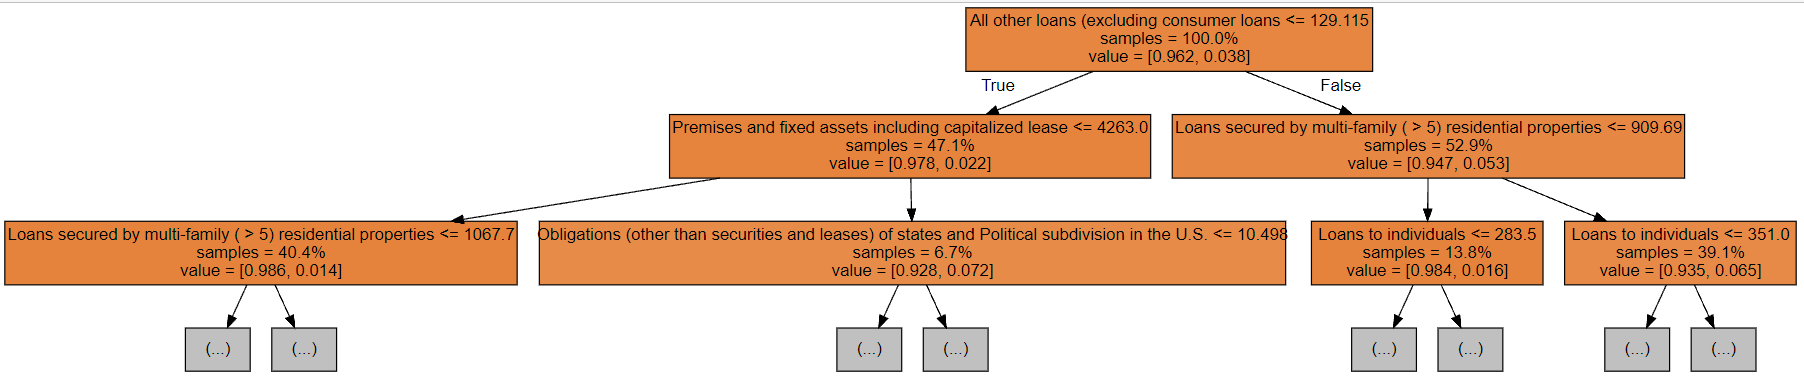
\includegraphics[width = \linewidth]{tree_1.png}
     \caption{Some examples of Classification Tree}\label{fig:tree_1}
\end{figure}

\begin{figure}[h]
     \centering
     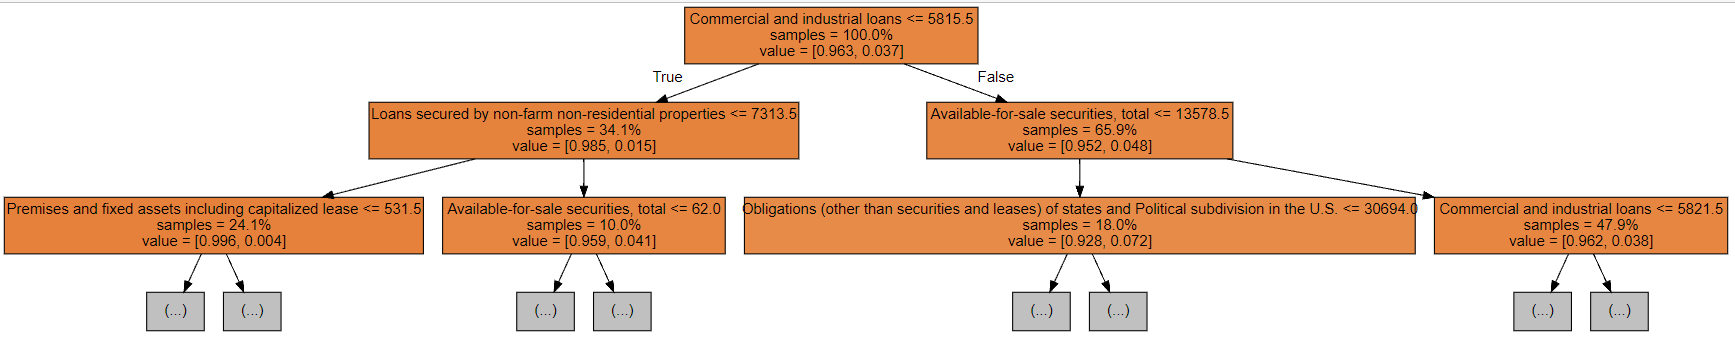
\includegraphics[width = \linewidth]{tree_2.png}
     \caption{Some examples of Classification Tree}\label{fig:tree_2}
\end{figure}

\begin{figure}[h]
     \centering
     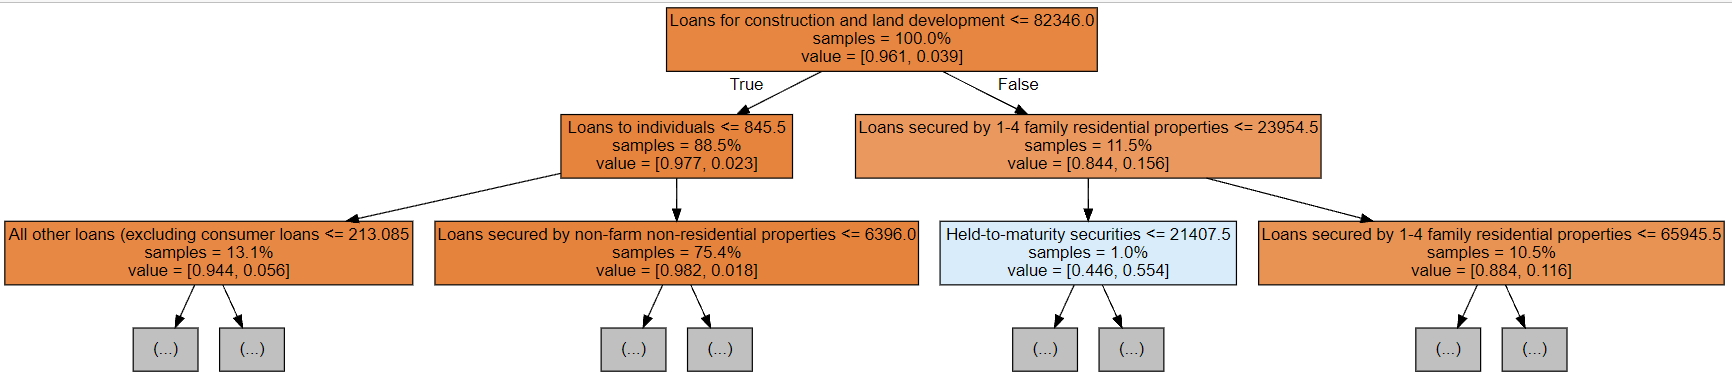
\includegraphics[width = \linewidth]{tree_3.png}
     \caption{Some examples of Classification Tree}\label{fig:tree_3}
\end{figure}
Here are some examples of classification trees. They shows the step of how the classification were made step by step.

\subsection{Method 3: Random Forest}
%https://easyai.tech/ai-definition/random-forest/
Random forest is an extended variant of Bagging. After understanding the Bagging method, random forest is much easier to learn. On the basis of building Bagging ensemble with decision tree as the base learner, RF further adds random attribute selection in the training process of decision tree. Specifically, the traditional decision tree selects an optimal attribute among all candidate attributes (assumed to be d) of the current node when selecting the partition attribute; while in RF, for each node of the base decision tree, first Randomly select a subset containing k attributes from the candidate attribute set of the node, and then select an optimal attribute from this subset for division. The selection of the number of attributes k to be extracted is more important, and is generally recommended. Therefore, the "diversity" of the base learner of the random forest comes not only from the perturbation of the samples, but also from the perturbation of the attributes, which further enhances the generalization ability of the final ensemble.

The main characteristics of random forest are: the individual learner is a decision tree, which samples the training samples and randomly samples the attributes.
\section{Analysis \& Results}

\subsection{Precision, Recall, F1 Score}

%https://thecleverprogrammer.com/2021/07/07/classification-report-in-machine-learning/#:~:text=A%20classification%20report%20is%20a,of%20your%20trained%20classification%20model.

%https://www.analyticsvidhya.com/blog/2019/08/11-important-model-evaluation-error-metrics/?utm_source=blog&utm_medium=decision-tree-vs-random-forest-algorithm

\begin{table}[h]
     \caption[table]{Report of Logistic Regression}
     \vspace{0.5em}\centering
     \begin{tabular}{ccccc}
         \toprule[1.5pt]
         &    precision    &recall  &f1-score   &support\\
         \midrule[1pt]                                   
         0       &0.97      &0.99      &0.98      &2243\\
         1       &0.41      &0.25      &0.31      &92\\
           & & & &                                   \\
  accuracy      &           &          &0.96      &2335\\
 macro avg      & 0.69      &0.62      &0.64      &2335\\
weighted avg    &   0.95    &  0.96    &  0.95    &  2335\\
         \bottomrule[1.5pt]
     \end{tabular}
\end{table}


\begin{table}[h]
     \caption[table]{Report of Classification Tree}
     \vspace{0.5em}\centering
     \begin{tabular}{ccccc}
         \toprule[1.5pt]
                &precision    &recall  &f1-score   &support\\
         \midrule[1pt]
         0      & 0.97      &0.96      &0.97      &2243\\
         1      & 0.22      &0.26      &0.24      &  92\\
         & & & &\\
  accuracy      &           &          &0.93      &2335\\
 macro avg      & 0.60      &0.61      &0.60      &2335\\
 weighted avg    &   0.94    & 0.93     & 0.94     & 2335\\
         \bottomrule[1.5pt]
     \end{tabular}
\end{table}

\subsection{ROC Curve}
ROC (Receiver Operating Characteristic) curve, also known as the receiver operating characteristic curve. This curve was first used in the field of radar signal detection to distinguish signal from noise. Later, people used it to evaluate the predictive ability of the model, and the ROC curve was derived based on the confusion matrix.

\begin{figure}[h]
     \centering
     \begin{minipage}{0.49\textwidth}
     \centering
     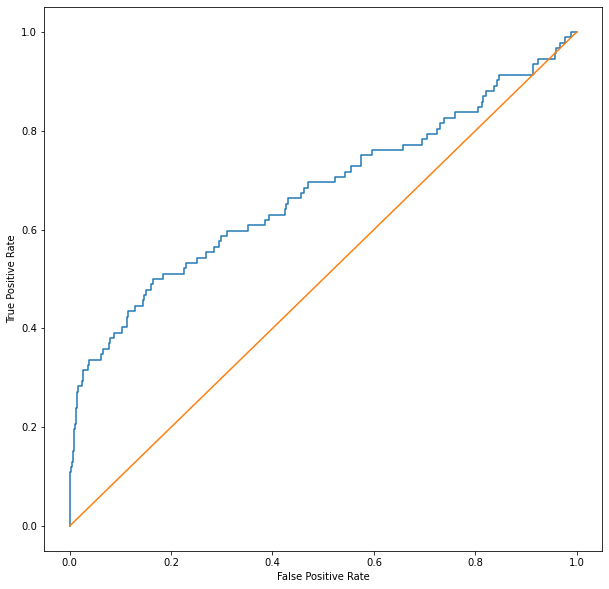
\includegraphics[width = \linewidth]{lr_roc.png}
     \caption{ROC Curve of Logistic Regression}\label{fig:lr_roc}
     \end{minipage}
     \centering
     \begin{minipage}{0.49\textwidth}
     \centering
     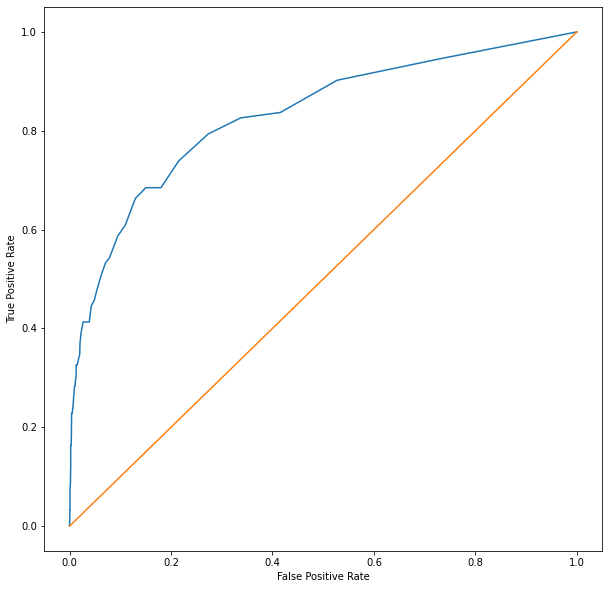
\includegraphics[width = \linewidth]{rf_roc.png}
     \caption{ROC Curve of Classification Tree}\label{fig:rf_roc}
     \end{minipage}
     \caption{ROC Curve}\label{fig:roc}
 \end{figure}

\subsection{AUC}

AUC (Area Under Curve) is defined as the area enclosed by the ROC curve and the coordinate axis. Obviously, the value of this area will not be greater than 1. And because the ROC curve is generally above the straight line y=x, the value range of AUC is between 0.5 and 1. The closer the AUC is to 1.0, the higher the authenticity of the detection method; when it is equal to 0.5, the authenticity is the lowest and has no application value.

Results:

Logistic Regression AUC: 0.6745769446975131

Classification Trees AUC: 0.6117098606292038

Random Forest AUC: 0.8128743530597609

As we can see, the AUC of Random Forest has the best performance, this is in line with the characteristics of Random Forest: reducing the number of trees and improving stability.

\subsection{Confusion Matrix}

The confusion matrix, also known as the error matrix, is a standard format for expressing accuracy evaluation, expressed in the form of a matrix with n rows and n columns. Specific evaluation indicators include overall accuracy, mapping accuracy, user accuracy, etc. These accuracy indicators reflect the accuracy of image classification from different aspects.

\begin{figure}[h]
     \centering
     \begin{minipage}{0.32\textwidth}
     \centering
     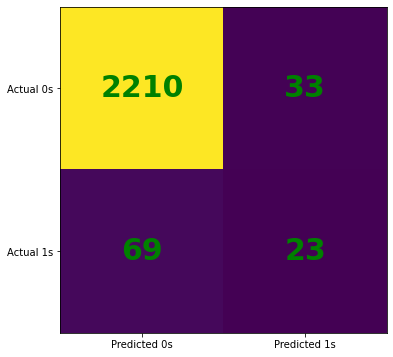
\includegraphics[width = \linewidth]{lr_cm.png}
     \caption{Confusion Matrix of Logistic Regression}\label{fig:lr_cm}
     \end{minipage}
     \centering
     \begin{minipage}{0.32\textwidth}
     \centering
     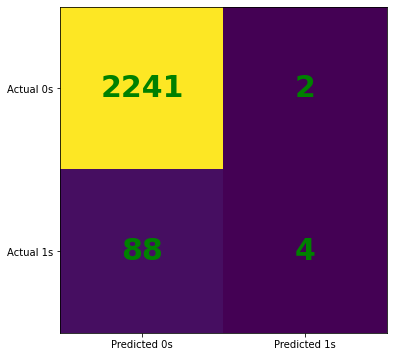
\includegraphics[width = \linewidth]{rf_cm.png}
     \caption{Confusion Matrix of Random Forests}\label{fig:rf_cm}
     \end{minipage}
     \centering
     \begin{minipage}{0.32\textwidth}
     \centering
     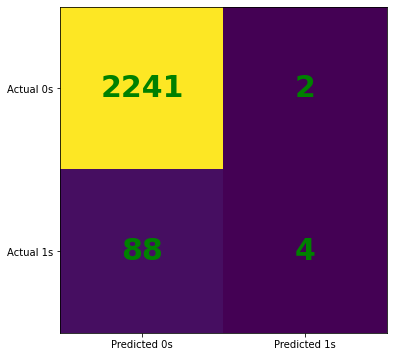
\includegraphics[width = \linewidth]{rs_cm.png}
     \caption{Confusion Matrix of Random Search}\label{fig:rs_cm}
     \end{minipage}
     \caption{Confusion Matrix}\label{fig:cm}
\end{figure}

The algorithm parameter solver = 'liblinear' result a accuracy of 95.63\%, while the solver = 'lbfgs' result a accuracy of 95.58\%, 'newton-cg' result a accuracy of 96.18\% but it warnings not converge. So the parameter I've choosed is the 'liblinear', which has almost no effect on the accuracy and is the most suitable algorithm in this predict model. The solver change has almost no effect on the accuracy.

Again, the Random Forest has the best performance, same reason as the ROC and AUC explanation, just because they are different aspect of the same performance, the relationship between predicted categories and real samples.

\subsection{Feature Importances}
Feature importance is a method of scoring input features to a predictive model that reveals the relative importance of each feature when making a prediction. Feature importance scores can be calculated for problems that involve predicting numeric values (called regression) and problems that involve predicting class labels (called classification).

\begin{figure}[h]
     \centering
     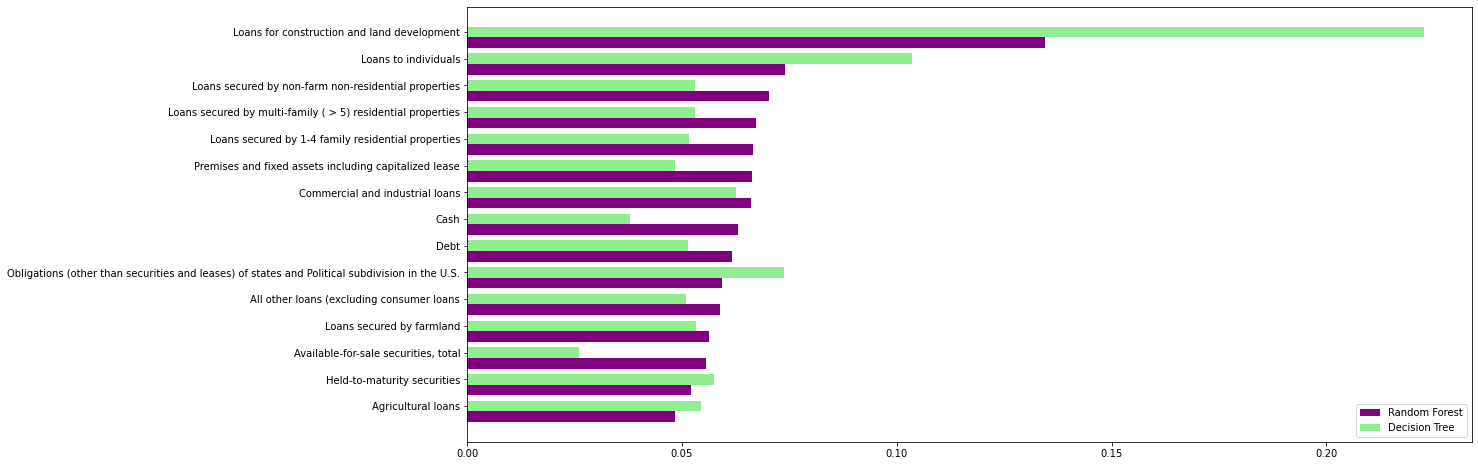
\includegraphics[width = \linewidth]{cf_rf_fi.png}
     \caption{Feature Importances of Classification Tree vs Random Forests}\label{fig:cf_rf_fi}
\end{figure}

\begin{figure}[h]
     \centering
     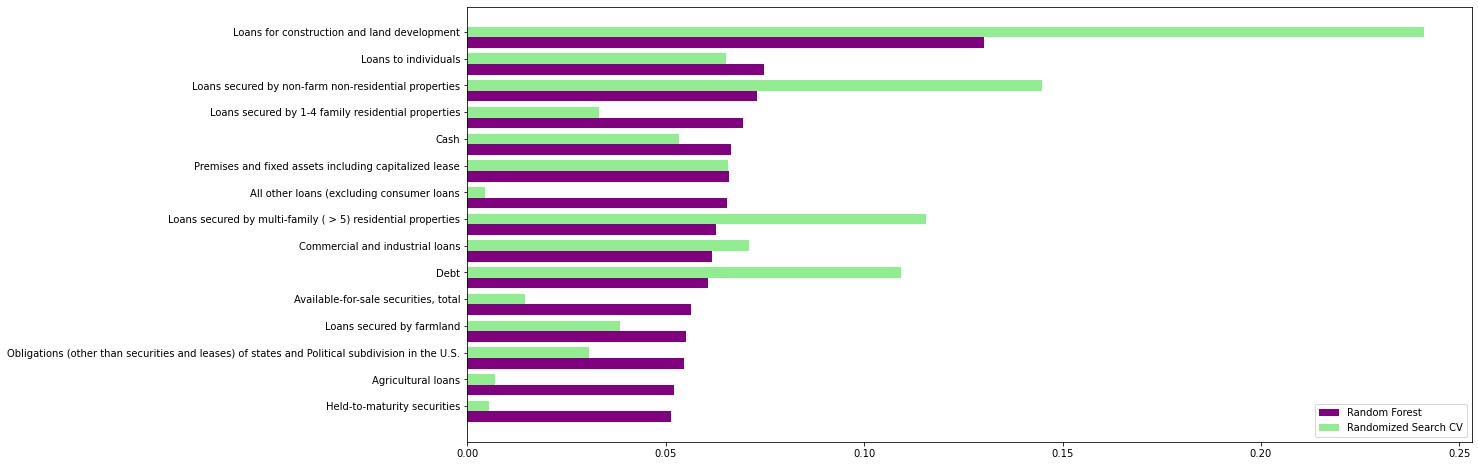
\includegraphics[width = \linewidth]{rf_rs_fi.png}
     \caption{Feature Importances of Random Forests vs Random Search}\label{fig:rf_rs_fi}
\end{figure}

It is easy to understand from this map that why Random Forests is more stable than Classification Tree, and the Random Search is more stable than Random Forests. The latter ones more average the weight of each feature, instead of focusing on only one of the variables.

\section{Discussion \& Conclusion}


\subsection{Interpretation of Results}
%https://www.analyticsvidhya.com/blog/2020/05/decision-tree-vs-random-forest-algorithm/
A decision tree is more simple and interpretable but prone to overfitting, but a random forest is complex and prevents the risk of overfitting.
Random forest is a more robust and generalized performance on new data, widely used in various domains such as finance, healthcare, and deep learning.

\subsection{Potential Limitations}

\subsubsection{Pros and Cons of Logistic Regression}
(Feature correlation situation) Because it is essentially a linear classifier, it does not handle the correlation between features well.
(Feature space) When the feature space is large, the performance is not good.
(Accuracy) It is easy to underfit and the accuracy is not high.

Stop condition:

The process of building a decision tree is a recursive process, so the stopping condition needs to be determined, otherwise the process will not end. One of the most intuitive ways is to stop when each child node has only one type of record, but this often makes the tree too many nodes, resulting in overfitting problems (Overfitting). Another feasible method is that the number of records in the current node is lower than a minimum threshold, then stop splitting, and use the classification corresponding to max(P(i)) as the classification of the current leaf node.
\subsubsection{Pros and Cons of Classification Trees}
Overfitting: The decision tree generated by the above algorithm often leads to overfitting in the event. That is, the decision tree can get a very low error rate for the training data, but it can get a very high error rate when applied to the test data. The reasons for the transition fit are as follows:

Noise data: There is noise data in the training data, and some nodes of the decision tree have noise data as the segmentation standard, which makes the decision tree unable to represent the real data.

Lack of representative data: The training data does not contain all representative data, resulting in a certain type of data that cannot be matched well, which can be obtained by observing the confusion matrix (Confusion Matrix).

Multiple comparison (Mulitple Comparison), this situation is similar to the selection of split points in decision trees. It is necessary to select one of each value of each variable as a split representative, so the probability of selecting a noise split standard is very high.

\subsubsection{Pros and Cons of Random Forests}

\textbf{Advantages:}

It can produce very high-dimensional (many features) data without dimensionality reduction or feature selection.

It can judge the importance of features.

Interactions between different features can be judged.

It is not easy to overfit.

The training speed is relatively fast, and it is easy to make a parallel method.

It is relatively simple to implement.

For unbalanced datasets, it can balances the errors.

Its accuracy can still be maintained if a large fraction of features are missing.

\textbf{Shortcomings:}

Random forests have been shown to overfit on some noisy classification or regression problems.

For data with attributes with different values, attributes with more value divisions will have a greater impact on random forests, so the attribute weights produced by random forests on such data are not credible.

\chapter{Task 2}
\section{Introduction}
In this part, I considered three approaches for a clustering analysis on the daily equity returns for 48 sectors in the US. This is unsupervised learning due to a lack of ground truth about how the sectors cluster together. The results of K-Means Algorithm and Hierarchical Clustering are given and compared below. However, the Expectation-Maximisation Algorithm is not suitable for multidimensional variables due to a high computation requirement. Besides, a PCA analysis on these independent variables is not required since I don't need to analyse the relationship between the independent variables of industries returns and a certain dependent variable. Some funny thing happened during my data cleaning process.

\section{Methodology}

\subsection{Data Cleaning}
I have to say that the data cleaning part is the most interesting part in these task. The dataset comes from Ken French's website and contains daily equity returns for 48 industries in the U.S.. I found that less than half of the days were missing data, so I want to drop that days and analyse the remain days. After I simply tried "df.dropna()" in python, nothing was happened. After a long period of debugging, I found that the labels of missing data were string type " NaN" instead of "np.nan()". When I solved this ridiculous bug, everything else goes sommthly. I clustered them into 5 parts and found some interpretations above them.

\subsection{Sample Selection}
Since I was going to analyse the return ability of all the industries, I could't cluster them by using their daily data, in row format. So the first thing for me is to transpose the matrix, or the dataframe, to let rows data becomes industries. Also, I was not intend to give up any industry so again I choose all the industries as my train data.

\subsection{Method 1: K-Means Algorithm}

%https://realpython.com/k-means-clustering-python/
The first method is based on the iteration of two steps: labelling the points and updating the centroids. For simplicity, I assume there are two clusters with centroids randomly initialised as $\mu_l, l=1, 2$. 

By solving $c^{(i)} = \text{arg}min_l \lVert x^{(i)} - \mu_l\rVert$, I can assign each point to its nearest cluster (either 1 or 2). Then I update the centroids with 

\[
     \mu_l=\frac{\sum_{i=1}^N x^{(i)}\mathds{1}\{c^{(i)}=l\}}{\sum_{i=1}^N\mathds{1}\{c^{(i)}=l\}}, 
\]

where $\mathds{1}\{c^{(i)}=l\}$ will be 1 if point $i$ belongs to cluster $l$, otherwise it will be zero. The steps are repeated until the update is below a threshold, i.e., convergence.

\subsection{Optimal Number Identification}
To figure out the optimal number of clusters, I use the cost function 
\[
     \mathbb{L}(c,\mu)=\sum_{i=1}^N \lVert x^{(i)}-\mu_c^{(i)}\rVert^2
\]   to measure the distance between the points and the centroids of their clusters. After clustering with larger number of clusters $(k=2,3,\cdots ,10)$,  I plot a graph of the value of the cost function after convergence against the number of clusters k, so that the optimal number can be identified, where the decrease in L by adding one cluster starts to drop, i.e., the “elbow”.

\subsection{Method 2: Expectation-Maximisation Algorithm}

The second method has the assumption that 
\[
     p(x^{(i)},c^{(i)})=p(x^{(i)}\mid c^{(i)})*p(c^{(i)}) 
\]
where 
\[
     p(x^{(i)}\mid c^{(i)}=l) \sim N(\mu_l, \sigma_l)
\] 
and 
\[
     p(c^{(i)}=l) \sim Multinomial(\phi_l ) 
\]
with random parameters. There are also two steps to be iterated until convergence. 

The E-step is to guess the labelling by computing the probability that a point belongs to a cluster, which is 
\begin{align*}
     \gamma_l^{(i)}&=p(c^{(i)}= l\mid x^{(i)} ;{\mu},{\sigma},{\phi})\\
     &=\frac{p(x^{(i)}\mid c^{(i)} = l)*p(c^{(i)}=l)}{p(x^{(i)})}
\end{align*}
Then, the M-step is to use the probabilities computed to update the parameters.

\subsection{Method 3: Hierarchical Clustering}
The last is a bottom-up method starting with each point labelled as its own cluster. This is proceeded by aggregation: merging the two closest points to form the first cluster, then the two closest clusters to form a larger cluster until all points belong to a big single cluster. The dissimilarity between points is measured by the Manhattan distance 

\begin{align*}
     d(i,j)=\sum_{k=1}^n|x_k^{(i)}-x_k^{(j)}|
\end{align*} , and the dissimilarity between clusters is dependent on the linkage criteria. Finally, the clustering can be shown by a dendrogram.

\section{Analysis \& Results}

\subsection{Result 1: K-Means}

\begin{figure}[h]
     \centering
     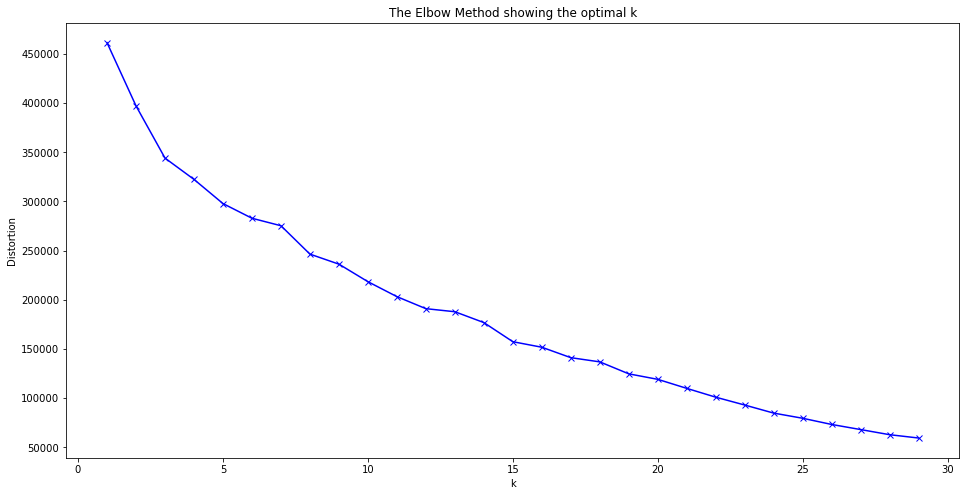
\includegraphics[width = \linewidth]{elbow.png}
     \caption{The elbow method showing the optimal method K}\label{fig:elbow}
\end{figure}

I found that the result of the k-means model under a fixed cluster numbers(I fixed it to 5) has a huge randomness. The result in each cluster was not equally distributed. Most of my results look likes this:

\begin{lstlisting}

Cluster 0 has industries: ['Smoke'] 
Cluster 1 has industries: ['Agric' 'Food ' 'Soda ' 'Beer ' 'Books' 'Hshld''Clths' 'Chems' 'Rubbr'
 'Txtls' 'BldMt' 'Cnstr' 'Steel' 'FabPr' 'Mach ' 'Autos' 'Aero ' 'Ships'
 'Guns ' 'Mines' 'Oil  ' 'Util ' 'PerSv' 'Paper' 'Boxes' 'Trans' 'Whlsl'
 'Rtail' 'Meals' 'Banks' 'Insur' 'RlEst' 'Fin  '] 

Cluster 2 has industries: ['Gold '] 

Cluster 3 has industries: ['Toys ' 'Fun  ' 'Hlth ' 'MedEq' 'Drugs' 'ElcEq''Telcm' 'BusSv' 'Comps'
 'Chips' 'LabEq' 'Other'] 

Cluster 4 has industries: ['Coal '] 

\end{lstlisting}

The rest clusters only have one industry. I noticed that the clusters that only contain 1 industries always contains the same set: Gold, Smoke, Coal, and sometimes Mines. Maybe those industries has very high return. Indeed, these industries might be all profitable. So I calculated their average return and sorted them. The resuld shows that the lowest 3 average return industries are Util: 676.25, Coal: 730.76 and Txtls: 742.59, while the highest 3 industries are Drugs: 1147.63, Gold: 1267.17 and LabEq: 1281.88. This is contradict to the clustering results.

\subsection{Result 2: Expectation-Maximisation Algorithm}
It was hard to deploy on a high dimensional data so I give up that.

\subsection{Result 3: Hierarchical Clustering}
\begin{figure}[h]
     \centering
     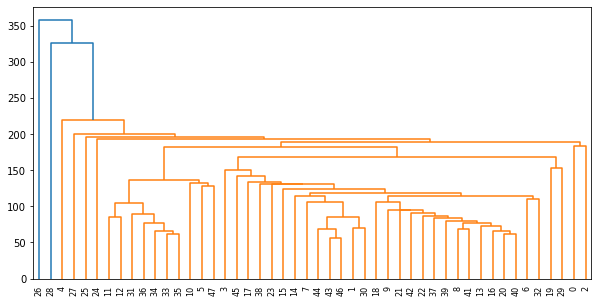
\includegraphics[width = \linewidth]{hc.png}
     \caption{Hierarchical Clustering Linkage}\label{fig:hc}
\end{figure}
\subsection{Performance Comparison}
The three results are approximately same.

\section{Discussion\& Conclusion}
\subsection{Potential Limitations}
\subsubsection{Pros and Cons of K-Means}
Advantages of K-Means:

The principle is simple and the convergence speed is fast, which is one of the important reasons why the industry uses it the most.

When tuning parameters, only one parameter k needs to be changed.

The principle of the algorithm is simple and interpretable.

Disadvantages of K-Means: 

Sensitive to outliers and noise points. For example, if you manually add a noise point far away from the center, the center position will be pulled far away.

The choice of k value is difficult to determine.

Only globular clusters can be found. In k-means, we use a single point to model the cluster, which actually assumes that the data of each cluster is distributed in a high-dimensional spherical shape, but the probability of this situation in life is not high. For example, each cluster is a long strip, and k-means cannot recognize this category at all (GMM can be used in this case). In fact, k-means is doing convex optimization, so it cannot handle non-convex distributions.

If the distance between the two categories is relatively close, the effect of k-means will not be very good.

The initial value has a great influence on the result, and the clustering result may be different every time.

The result may be only a local optimum rather than a global optimum.

\subsubsection{Pros and Cons of Hierarchical Clustering}
Advantage:
1. The similarity between distance and rules is easy to define, with few restrictions.

2. There is no need to pre-specify the number of clusters.

3. You can discover the hierarchical relationship of classes.

Shortcoming:

1. The computational complexity is too high.

2. Singular values can also have a great impact.

3. The algorithm is likely to cluster into a chain.



\end{document}